\documentclass[11pt]{article}
\usepackage{amsmath}
\usepackage{listings}
\usepackage{graphicx}


\begin{document}
\title{PHY 480 Project 1}
\author{Benjamin Brophy}
\maketitle

\section{Abstract}
In this project I will use both the Verlet Method and the Runge Kutta Method to produce a model of the solar system, based only on gravitational force and the properties of the planets. Both methods produced results which accurately mapped the solar system.

\section{Introduction}
The gravitational force between two objects is represented by 
$$F = \frac{GMm}{r^2}$$ where G is the gravitational constant, M is the mass of the larger object, and r is the distance between the two objects.
The only forces acting on an objects in space are the gravitational pulls of other planets or stars. If a planet is in a circular orbit around the sun, then this force will be equal to the centripetal force of an object in circular motion.
$$F = \frac{mv^2}{r}$$
For an object in circular motion around the Sun with mass M, we then find 
$$GM = v^2r$$
which is constant. Then we can taking the Earth as an example, we know that the Earth has a radius defined as 1 AU, and the velocity is the circumference of Earth's circular orbit divided by one year. $v=(2\pi $AU$)/yr$ and
$$GM = 4\pi^2 AU^3/yr^2$$

Also, we know Newton's second law is $F=ma$ where a is acceleration of a planet. Thus the acceleration of a planet around the sun, or derivative of a planet's velocity, will be
$$\frac{dv}{dt} = a = -\frac{GM}{r^2} =-\frac{4\pi^2}{r^2} $$

Taking our mass units as solar masses, we can find the acceleration of a planet due to any other planet with the following formula
$$\frac{dv}{dt} = a = -\frac{4\pi^2M}{r^2} $$

One can think of M as either the orbited planet's mass in solar masses, or the ratio of the orbited planet's mass to the sun.

Since $\vec{r}=x\hat{x}+y\hat{y}$ we can break the force into two components,

$$
F_{x} = -\frac{4\pi^2Mm\Delta x}{r^{3}}\text{ and } F_{y} = -\frac{4\pi^2Mm\Delta y}{r^{3}}
$$
where $\Delta x$ and $\Delta y$ are difference in x and y coordinates of the planets, respectively.
We obtain two coupled second-order differential equations:

\begin{equation}
\label{eq:diffeqs1}
a_x=\frac{d^{2}x}{dt^{2}} = -\frac{4\pi^2Mx}{r^{3}}\text{ and } a_y = \frac{d^{2}y}{dt^{2}} = -\frac{4\pi^2My}{r^{3}}
\end{equation}

The escape velocity for an object with mass m orbiting an object of mass M can be found by equating gravitational potential energy and kinetic energy.
$$\frac{GMm}{r} = \frac{1}{2}mv_e^2$$
$$v_e=\sqrt{\frac{2GM}{r}}$$

For a planet at Earth's orbit, of any mass, this velocity should then be
$$v_e = \sqrt{8\pi^2} AU/yr = 8.89 AU/yr$$

Below this velocity, no matter what speed an direction, the orbiting object should still orbit the Sun in an ellipse. Once the object reaches escape velocity, it should follow a parabolic path away from the Sun.

\section{Methods}

The Verlet method is a method of approximation obtained by Taylor expanding the position and velocity of an object. If we discretize our differential equations into N equally spaced points labeled i from 0 to N, where $x_i$ is a position and $v_i$ is the velocity at that position, and $a_i$ is the acceleration at that position, the Verlet method algorithm is as follows:

$$x_{i+1}=x_i+hv_i + h^2/2 * a_i$$
$$v_{i+1}=v_i+h/2(a_i+a_{i+1})$$

We can implement this for each direction since the x and y directions are independent from each other in our equations. (Technically, r depends on both x and y, but we treat it as a constant for each step of the calculation)


For the Runge Kutta method, one can find the approximate discretized values of a function by integrating a known derivative of our function and Taylor expanding this integral. The fourth order Runge-Kutta gives us the following algorithm for each step of a function g with derivative f:
$$k_1 = hf(t_i,g_i)$$
$$k_2 = hf(t_i+h/2,g_i + k_1/2)$$
$$k_3 = hf(t_i + h/2,g_i + k_2/2)$$
$$k_4 = hf(t_i + h, g_i+k_3)$$
$$g_{i+1} = g_i + (k_1 + 2k_2 + 2k_3 + k_4)/6$$

Since we are calculating both position and velocity at the same time, and we know the expression for acceleration $a_i=a(x_i)$ dependent on position, we rewrite these equations in this fashion, where x is added to the subscript of a position and v is added to the subscript for a velocity:

$$k_{1x} = hv_i$$
$$k_{1v} = ha_i$$

$$k_{2x} = h(v_i+k_{1v}/2)$$
$$k_{2v} = ha(x_i+k_{1x}/2)$$
$$k_{3x} = h(v_i+k_{2v}/2)$$
$$k_{3v} = ha(x_i+k_{2x}/2)$$
$$k_{4x} = h(v_i+k_{3v})$$
$$k_{4v} = ha(x_i+k_{3x})$$

$$x_{i+1} = x_i + (k_{1x} + 2k_{2x} + 2k_{3x} + k_{4x})/6$$
$$v_{i+1} = v_i + (k_{1v} + 2k_{2v} + 2k_{3v} + k_{4v})/6$$

I implemented two classes. One was a planet class, which stored the name of the planet, position vector, and velocity vector for the planet. It contains functions which calculate the distance between any two planets, and to perform either the Verlet method or RK4 method to approximate the planet orbiting the Sun for a given number of points per Earth year and number of years.

I also implemented an "asystem" class. An object in asystem has an associated list of planets, number of planets, and total mass of all planets. It has functions to add a planet to the planet list, center all the planets at the center of mass of the system, and calculate the orbit of all planets using the Verlet method.

\section{Results and Analysis}
In Figure 1, we model Earth orbiting a static sun for 5 years using the Verlet method, with each year having 100 discrete points. After this time, Earth is still in a stable orbit, only decreasing its distance from the sun by .5\%.

\begin{figure}
	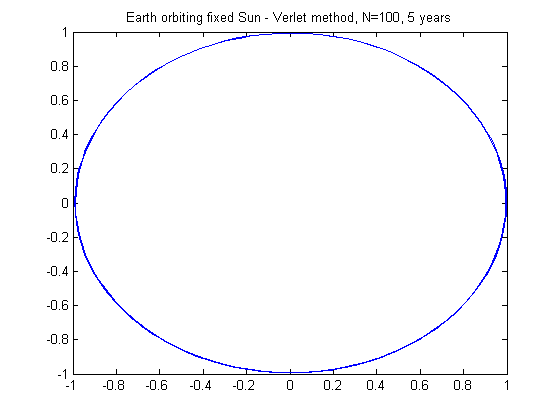
\includegraphics[width=\linewidth]{EarthverletN100yr5}
	\caption{Axes are in AU, with Sun at (0,0)}
\end{figure}
 
In Figure 2,  we model Earth orbiting a static sun for 5 years using the RK4 method, with each year having 100 discrete points. After this time, Earth is still in a stable orbit, only decreasing its distance from the sun by .57\%.

\begin{figure}
	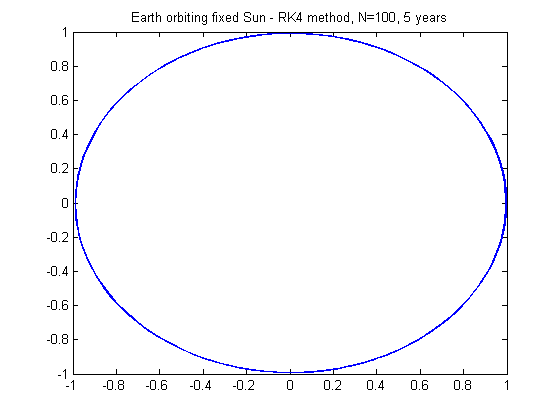
\includegraphics[width=\linewidth]{Earthrk4N100yr5}
	\caption{Axes are in AU, with Sun at (0,0)}
\end{figure}

Next we explore escape velocity. I incrementally increased the orbital velocity of an object at 1 AU from the sun by 0.1 AU/yr and observed the orbits calculated by the RK4 method. As expected, once the object passed the 8.89 AU/yr escape velocity of the Sun at 1 AU, the object followed a parabolic path away from the Sun. See Figure 3.

\begin{figure}
	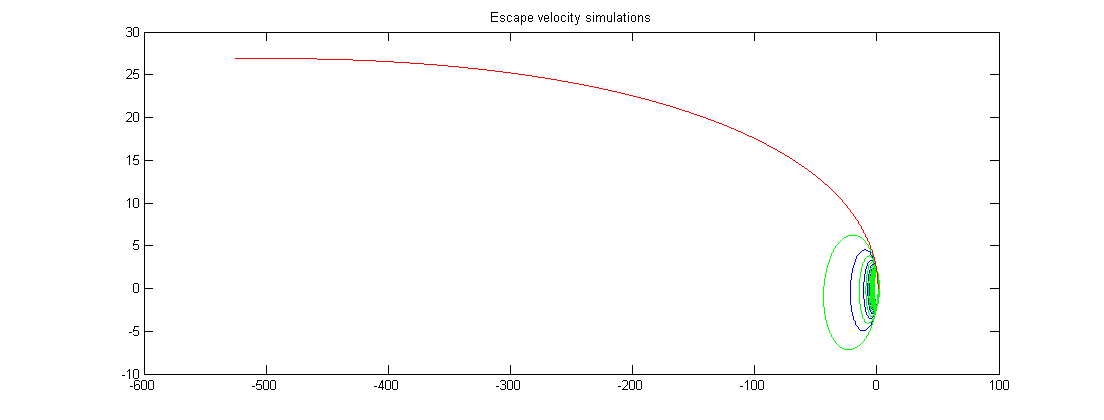
\includegraphics[width=\linewidth]{escape}
	\caption{Axes are in AU, with Sun at (0,0). In blue is the path of a planet starting 1 AU from the Sun with a velocity of 8.7 AU/yr for 256 years. In green is the path of a planet starting 1 AU from the Sun with a velocity of 8.8 AU/yr for 512 years. In red is the path of a planet starting 1 AU from the Sun with a velocity of 8.9 AU/yr for 256 years.}
\end{figure}

Finally, here we model the entire solar system with the Verlet method. We first look at the interior planets on the scale of 10 years in Figure 4. The orbits are stable and accurate on this short time frame. Because Pluto's orbit takes about 250 years, we plotted over the course of 250 years to capture the whole solar system in Figure 5. The center planets and the sun are not stable over 250 years but the outer planets have accurate orbits.

\begin{figure}
	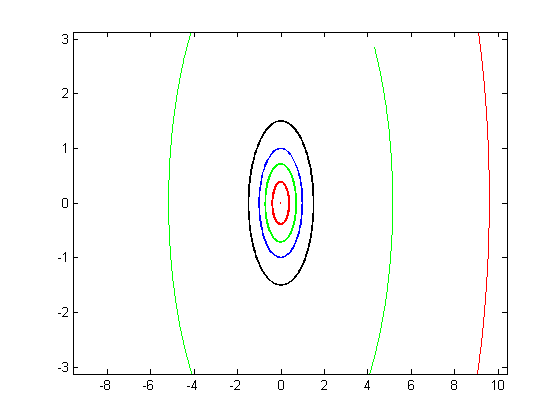
\includegraphics[width=\linewidth]{n100yr10}
	\caption{Axes are in AU, with the center of mass at (0,0). The Solar System generated with the Sun, all 8 planets, and Pluto. N = 100, yr = 10.}
\end{figure}

\begin{figure}
	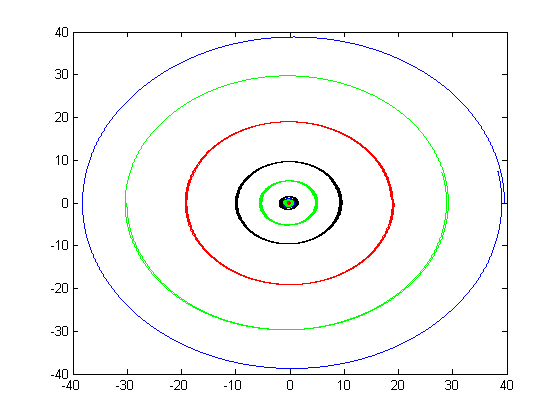
\includegraphics[width=\linewidth]{n200yr250}
	\caption{Axes are in AU, with the center of mass at (0,0.  The Solar System generated with the Sun, all 8 planets, and Pluto. N = 100, yr = 10.)}
\end{figure}


\section{Bibliography}
[1] Hjorth-Jensen, Morten. "Computational Physics Lectures: Ordinary Differential Equations." Mathematics of Computation (n.d.): n. pag. Web.
[2] Sauer, Tim. Numerical Analysis. Boston: Pearson, 2012. Print.

\section{Code}

\begin{verbatim}
#include <iostream>
#include <math.h>
#include <fstream>
#include <string>
#include <vector>

using namespace std;

class planet {
public:
double position[2];
double velocity[2];
double mass;
std::string name;
planet(std::string planetname, double M, double x,double y, double vx, double vy);
planet();
double distance(planet other);
void rk4method1(int N, int years);
void verletmethod1(int N, int years);
};

planet::planet(std::string planetname, double M, double x, double y, double vx, double vy){
name = planetname;
mass = M;
position[0]=x; //position in AU
position[1] = y;
velocity[0] = vx; //velocities in AU/yr
velocity[1] = vy;
};

double planet::distance(planet other){
double xdiff = position[0]-other.position[0];
double ydiff = position[1]-other.position[1];
double r = sqrt(xdiff*xdiff+ydiff*ydiff);
return r;
};

void planet::rk4method1(int N, int years){
cout<<"rk4method"<<endl;
double PI = 3.141526535;
double n = N;
double h = 1/(1+n);
std::string N_str = std::to_string(N);
std::string yr_str = std::to_string(years);
std::string filename = "rk4method1/"+name+"rk4" + "N" + N_str +"yr" + yr_str + ".csv";
ofstream myfile (filename);

if (myfile.is_open())
{
planet Sun("Sun",1,0,0,0,0);
double t=0; //time in years
double x = position[0];
double vx = velocity[0];
double y = position[1];
double vy = velocity[1];
double r;
//double x1, vx1, y1, vy1;
double k1x, k1vx, k1y,k1vy;
double k2x, k2vx, k2y,k2vy;
double k3x, k3vx, k3y,k3vy;
double k4x, k4vx, k4y,k4vy;


//cout << t<< x<< vx << y << vy<< "\n" ;
myfile << t << ","<< x<< ","<< vx<< "," << y<< "," << vy<< "\n" ;
for(int count = 0; count <= (years*N); count ++){
r = distance(Sun);
t = t + h;
//k1
k1x = h*vx;
k1vx = -4*PI*PI*x*h/(r*r*r);
k1y = h*vy;
k1vy = -4*PI*PI*y*h/(r*r*r);

//k2
k2x = h*(vx+k1vx/2);
k2vx = h*(-4*PI*PI)*(x+k1x/2)/(r*r*r);
k2y = h*(vy+k1vy/2);
k2vy = h*(-4*PI*PI)*(y+k1y/2)/(r*r*r);

//k3
k3x = h*(vx+k2vx/2);
k3vx = h*(-4*PI*PI)*(x+k2x/2)/(r*r*r);
k3y = h*(vy+k2vy/2);
k3vy = h*(-4*PI*PI)*(y+k2y/2)/(r*r*r);

//k4
k4x = h*(vx+k3vx);
k4vx = h*(-4*PI*PI)*(x+k3x)/(r*r*r);
k4y = h*(vy+k3vy);
k4vy = h*(-4*PI*PI)*(y+k3y)/(r*r*r);

x = x + (k1x + 2*k2x + 2 * k3x + k4x)/6;
vx = vx + (k1vx + 2*k2vx + 2 * k3vx + k4vx)/6;
y = y + (k1y + 2*k2y + 2 * k3y + k4y)/6;
vy = vy + (k1vy + 2*k2vy + 2 * k3vy + k4vy)/6;

myfile << t << ","<< x<< ","<< vx<< "," << y<< "," << vy<< "\n" ;
position[0] = x; //position in AU
position[1] = y;
velocity[0] = vx; //velocities in AU/yr
velocity[1] = vy;
}
myfile.close();
cout<<"Output to rkmethod1/..."<<endl;
position[0] = x; //position in AU
position[1] = y;
velocity[0] = vx; //velocities in AU/yr
velocity[1] = vy;
}

}

void planet::verletmethod1(int N, int years){
planet Sun("Sun",1,0,0,0,0);
double PI = 3.141526535;
double n = N;
double h = 1/(1+n);
std::string N_str = std::to_string(N);
std::string yr_str = std::to_string(years);
std::string filename = name+"verlet" + "N" + N_str +"yr" + yr_str + ".csv";
ofstream myfile (filename);
if (myfile.is_open()){
double t = 0.0; //time in years
double x = position[0];
double vx =velocity[0];
double y = position[1];
double vy = velocity[1];
double x1, vx1, y1, vy1, r;

//cout << t<< x<< vx << y << vy<< "\n" ;
myfile << t << ","<< x<< ","<< vx<< "," << y<< "," << vy<< "\n" ;
for(int count = 0; count <= (years*N); count ++){
r = distance(Sun);
//cout<<r;
t = t + h;
x1 = x + h*vx - h*h*2*PI*PI*x/(r*r*r);
vx1 = vx - 2*PI*PI*(x+x1)*h/(r*r*r);
y1 = y + h*vy - h*h*2*PI*PI*y/(r*r*r);
vy1 = vy - 2*PI*PI*(y+y1)*h/(r*r*r);
x= x1;
vx=vx1;
y=y1;
vy=vy1;
myfile << t << ","<< x<< ","<< vx<< "," << y<< "," << vy<< "\n" ;
position[0] = x; //position in AU
position[1] = y;
velocity[0] = vx; //velocities in AU/yr
velocity[1] = vy;
}
myfile.close();
cout<<"Output saved to "<<filename<<endl;
}

}

class asystem{
public:
vector<planet> planlist;
asystem();
int size;
double totmass;
void addplanet(planet plan);
void center(); //will automatically center masses at origin
void verletmethod(int N, int years);
void rk4method(int N, int years);

};

asystem::asystem(){
size = 0;
totmass = 0.0;
}

void asystem::addplanet(planet plan){
planlist.push_back(plan);
size++;
totmass += plan.mass;
};

void asystem::center(){
double xtot=0;
double ytot=0;
int i;
for(i=0; i < size ; i++){
planet plan = planlist[i];
xtot+= plan.position[0]*plan.mass;
ytot+= plan.position[1]*plan.mass;
}
double xcom = xtot/totmass;
double ycom = ytot/totmass;

for(i=0; i < size ; i++){
planet plan = planlist[i];
plan.position[0]-xcom;
plan.position[1]-ycom;
}

};

void asystem::verletmethod(int N, int years){
double PI = 3.141526535;
double n = N;
double h = 1/(1+n);
int i,j;
std::string N_str = std::to_string(N);
std::string yr_str = std::to_string(years);
double t = 0.0; //time in years
for(int count = 0; count < (years*N); count ++){ //iterate through number of steps
//cout << "count: "<<count;
for(i=0; i < size ; i++){               //iterate through eachplanet once per step
t = h*count;
//cout<<"Main: "<< plan.name;
std::string filename = "verlet2/sys"+planlist[i].name+"N"+N_str+"yr"+yr_str+"verlet.csv";
ofstream myfile (filename, std::ios::app);
double x1, y1, vx1, vy1, r;
//
x1 = planlist[i].position[0] + h*planlist[i].velocity[0];
y1 = planlist[i].position[1] + h*planlist[i].velocity[1];
vx1 = planlist[i].velocity[0];
vy1 = planlist[i].velocity[1];
for(j=0; j < size ; j++){     //for each other planet

if (i!=j){
planet plan2 = planlist[j];
r = planlist[i].distance(plan2);
x1 -= plan2.mass*h*h*2*PI*PI*(planlist[i].position[0]-plan2.position[0])/(r*r*r);
y1 -= plan2.mass*h*h*2*PI*PI*(planlist[i].position[1]-plan2.position[1])/(r*r*r);
//                           cout << "+"<<plan2.name<<endl;
//                           cout<<"change"<<h*h*2*PI*PI*(planlist[i].position[0]-plan2.position[0])/(r*r*r);
//                           cout <<"x1 after"<<x1<<endl;
}
}
for(j=0; j < size ; j++){     //for each other planet
if (i!=j){
planet plan2 = planlist[j];
//cout << "+"<<plan2.name<<endl;
r = planlist[i].distance(plan2);
//cout <<"vx1 before"<<vx1;
vx1 -= plan2.mass*2*PI*PI*(planlist[i].position[0]+x1-2*plan2.position[0])*h/(r*r*r);
//cout<<"change"<<4*PI*PI*(plan.position[0]-plan2.position[0])*h/(r*r*r);
//cout <<"vx1 after"<<vx1<<endl;
vy1 -= plan2.mass*2*PI*PI*(planlist[i].position[1]+y1-2*plan2.position[1])*h/(r*r*r);

}
}
planlist[i].position[0]=x1;
planlist[i].position[1]=y1;
planlist[i].velocity[0]=vx1;
planlist[i].velocity[1]=vy1;
myfile << t << ","<< x1 << ","<< vx1<< "," << y1<< "," << vy1<< "\n" ;
//cout << t << ","<< x1 << ","<< vx1<< "," << y1<< "," << vy1<< "\n" ;
myfile.close();

}
}
cout<<"Output saved to verlet2/..."<<endl;
}

void asystem::rk4method(int N, int years){
double PI = 3.141526535;
double n = N;
double h = 1/(1+n);
int i,j;
std::string N_str = std::to_string(N);
std::string yr_str = std::to_string(years);
double t = 0.0; //time in years
for(int count = 0; count < (years*N); count ++){ //iterate through number of steps
//cout << "count: "<<count;
for(i=0; i < size ; i++){               //iterate through eachplanet once per step
t = h*count;
//cout<<"Main: "<< plan.name;
std::string filename = "rk4method2/sys"+planlist[i].name+"N"+N_str+"yr"+yr_str+"verlet.csv";
ofstream myfile (filename, std::ios::app);
double x1, y1, vx1, vy1, r;
//
x1 = planlist[i].position[0] + h*planlist[i].velocity[0];
y1 = planlist[i].position[1] + h*planlist[i].velocity[1];
vx1 = planlist[i].velocity[0];
vy1 = planlist[i].velocity[1];
for(j=0; j < size ; j++){     //for each other planet

if (i!=j){
planet plan2 = planlist[j];
r = planlist[i].distance(plan2);
x1 -= plan2.mass*h*h*2*PI*PI*(planlist[i].position[0]-plan2.position[0])/(r*r*r);
y1 -= plan2.mass*h*h*2*PI*PI*(planlist[i].position[1]-plan2.position[1])/(r*r*r);
//                           cout << "+"<<plan2.name<<endl;
//                           cout<<"change"<<h*h*2*PI*PI*(planlist[i].position[0]-plan2.position[0])/(r*r*r);
//                           cout <<"x1 after"<<x1<<endl;
}
}
for(j=0; j < size ; j++){     //for each other planet
if (i!=j){
planet plan2 = planlist[j];
//cout << "+"<<plan2.name<<endl;
r = planlist[i].distance(plan2);
//cout <<"vx1 before"<<vx1;
vx1 -= plan2.mass*2*PI*PI*(planlist[i].position[0]+x1-2*plan2.position[0])*h/(r*r*r);
//cout<<"change"<<4*PI*PI*(plan.position[0]-plan2.position[0])*h/(r*r*r);
//cout <<"vx1 after"<<vx1<<endl;
vy1 -= plan2.mass*2*PI*PI*(planlist[i].position[1]+y1-2*plan2.position[1])*h/(r*r*r);

}
}
planlist[i].position[0]=x1;
planlist[i].position[1]=y1;
planlist[i].velocity[0]=vx1;
planlist[i].velocity[1]=vy1;
myfile << t << ","<< x1 << ","<< vx1<< "," << y1<< "," << vy1<< "\n" ;
//cout << t << ","<< x1 << ","<< vx1<< "," << y1<< "," << vy1<< "\n" ;
myfile.close();

}
}
cout<<"Output saved to verlet2/..."<<endl;
}




//void publishvector (double* X, int N, std::string filename){
////print vector X of size N with name "filename"
//    ofstream myfile (filename);
//    if (myfile.is_open())
//      {
//        for(int count = 0; count < N; count ++){
//            myfile << X[count] << "\n" ;
//        }
//        myfile.close();
//      }

//};

int main()
{
const double PI = 3.1415926535;
planet Sun("Sun",1,0,0,0,0);
planet Mercury("Mercury",1.2e-7, 0, .39,-9.960,0);
planet Venus("Venus",2.4e-6,-.72,0,0,7.36);
planet Earth("Earth",1.5e-6,1,0,0, 6.26);
planet Mars("Mars",3.3e-7, 1.52, 0,0,5.06);
planet Jupiter("Jupiter",9.5e-4, 0,5.20,-2.75,0);
planet Saturn("Saturn",2.75e-4, 0,-9.54,2.04,0);
planet Uranus("Uranus",4.4e-5, 19.19, 0,0,-1.43);
planet Neptune("Neptune",5.1e-5, -30.06, 0,0,-1.14);
planet Pluto("Pluto",5.6e-9, 39.53, 0,0,0.99);


//cout << "N?" << endl; //size of matrix
int N, i;
N = 10;
int years = 1;
double h;
//cin >> N;
double n = N;
h = 1/(n+1);
//    double *X = new double[N];
//    // initialize X array all elements = 2
//    for(i=0 ; i < N ; i++) {
//        X[i] = 2.0;}
//    std::string N_str = std::to_string(N);
//    std::string filename = "N" + N_str + ".txt";
//    publishvector(X,N,filename);

//partbverlet
if (false){
//verlet for earth
Earth.verletmethod1(100,5);

}

//partbRK4
if (false){
//rk4 for earth
planet Earth("Earth",1.5e-6,1,0,0, 6.26);
cout<<"hello"<<endl;
Earth.rk4method1(100,5);
cout<<"world"<<endl;
//       ofstream myfile ("earthrk4.csv");
//       if (myfile.is_open())
//         {

//           double t=0; //time in years
//           double x = Earth.position[0];
//           double vx = Earth.velocity[0];
//           double y = Earth.position[1];
//           double vy = Earth.velocity[1];
//           double r;
//           //double x1, vx1, y1, vy1;
//           double k1x, k1vx, k1y,k1vy;
//           double k2x, k2vx, k2y,k2vy;
//           double k3x, k3vx, k3y,k3vy;
//           double k4x, k4vx, k4y,k4vy;

//           //cout << t<< x<< vx << y << vy<< "\n" ;
//           myfile << t << ","<< x<< ","<< vx<< "," << y<< "," << vy<< "\n" ;
//           for(int count = 0; count < (years*N); count ++){
//               r = Sun.planet::distance(Earth);
//               t = t + h;
//               //k1
//               k1x = h*vx;
//               k1vx = -4*PI*PI*x*h/(r*r*r);
//               k1y = h*vy;
//               k1vy = -4*PI*PI*y*h/(r*r*r);

//               //k2
//               k2x = h*(vx+k1vx/2);
//               k2vx = h*(-4*PI*PI)*(x+k1x/2)/(r*r*r);
//               k2y = h*(vy+k1vy/2);
//               k2vy = h*(-4*PI*PI)*(y+k1y/2)/(r*r*r);

//               //k3
//               k3x = h*(vx+k2vx/2);
//               k3vx = h*(-4*PI*PI)*(x+k2x/2)/(r*r*r);
//               k3y = h*(vy+k2vy/2);
//               k3vy = h*(-4*PI*PI)*(y+k2y/2)/(r*r*r);

//               //k4
//               k4x = h*(vx+k3vx);
//               k4vx = h*(-4*PI*PI)*(x+k3x)/(r*r*r);
//               k4y = h*(vy+k3vy);
//               k4vy = h*(-4*PI*PI)*(y+k3y)/(r*r*r);

//               x = x + (k1x + 2*k2x + 2 * k3x + k4x)/6;
//               vx = vx + (k1vx + 2*k2vx + 2 * k3vx + k4vx)/6;
//               y = y + (k1y + 2*k2y + 2 * k3y + k4y)/6;
//               vy = vy + (k1vy + 2*k2vy + 2 * k3vy + k4vy)/6;

//               myfile << t << ","<< x<< ","<< vx<< "," << y<< "," << vy<< "\n" ;
//           }
//           myfile.close();
//         }
}
//end of partbrk4

//part d escape velocity
if (false){
float v = 8.0; //AU/YR
for(i=0; i < 11 ; i++){
cout<<i;
float vy = v+i*.1;
std::string i_str = std::to_string(i);
std::string planetname = "test"+i_str;
planet test(planetname,1000,1,0,0,vy);
test.rk4method1(100,pow(2,i));

}





};

//part f

if(true){
asystem solar;

solar.addplanet(Sun);
solar.addplanet(Mercury);
solar.addplanet(Venus);
solar.addplanet(Earth);
solar.addplanet(Mars);
solar.addplanet(Jupiter);
solar.addplanet(Saturn);
solar.addplanet(Uranus);
solar.addplanet(Neptune);
solar.addplanet(Pluto);

solar.center();
cout<<"size"<<solar.size<<endl;
solar.verletmethod(200,250);
};
system("pause");
}

\end{verbatim}
\end{document}